\documentclass[12pt,a4paper]{article}

\usepackage[a4paper,text={16.5cm,25.2cm},centering, margin=1in]{geometry}

\usepackage[scale=0.95]{FiraMono}
\usepackage[utf8]{inputenc}
\usepackage[T1]{fontenc}
\usepackage{mathpazo}

\usepackage{amssymb,amsmath}
\usepackage{bm}
\usepackage{graphicx}
\usepackage{microtype}
\usepackage{hyperref}
\setlength{\parindent}{0pt}
\setlength{\parskip}{1.2ex}

\usepackage{fvextra}
\DefineVerbatimEnvironment{Highlighting}{Verbatim}{breaklines,commandchars=\\\{\}}

\setcounter{secnumdepth}{0}

\hypersetup
       {   pdfauthor = { Ian Shen-Costello (iys2) },
           pdftitle={ BEE 4750/5750 Homework 3 },
           colorlinks=TRUE,
           linkcolor=black,
           citecolor=blue,
           urlcolor=blue
       }

\title{ BEE 4750/5750 Homework 3 }

\author{ Ian Shen-Costello (iys2) }

\date{ 2022-10-20 }

\usepackage{upquote}
\usepackage{listings}
\usepackage{xcolor}
\lstset{
    basicstyle=\ttfamily\footnotesize,
    upquote=true,
    breaklines=true,
    breakindent=0pt,
    keepspaces=true,
    showspaces=false,
    columns=fullflexible,
    showtabs=false,
    showstringspaces=false,
    escapeinside={(*@}{@*)},
    extendedchars=true,
}
\newcommand{\HLJLt}[1]{#1}
\newcommand{\HLJLw}[1]{#1}
\newcommand{\HLJLe}[1]{#1}
\newcommand{\HLJLeB}[1]{#1}
\newcommand{\HLJLo}[1]{#1}
\newcommand{\HLJLk}[1]{\textcolor[RGB]{148,91,176}{\textbf{#1}}}
\newcommand{\HLJLkc}[1]{\textcolor[RGB]{59,151,46}{\textit{#1}}}
\newcommand{\HLJLkd}[1]{\textcolor[RGB]{214,102,97}{\textit{#1}}}
\newcommand{\HLJLkn}[1]{\textcolor[RGB]{148,91,176}{\textbf{#1}}}
\newcommand{\HLJLkp}[1]{\textcolor[RGB]{148,91,176}{\textbf{#1}}}
\newcommand{\HLJLkr}[1]{\textcolor[RGB]{148,91,176}{\textbf{#1}}}
\newcommand{\HLJLkt}[1]{\textcolor[RGB]{148,91,176}{\textbf{#1}}}
\newcommand{\HLJLn}[1]{#1}
\newcommand{\HLJLna}[1]{#1}
\newcommand{\HLJLnb}[1]{#1}
\newcommand{\HLJLnbp}[1]{#1}
\newcommand{\HLJLnc}[1]{#1}
\newcommand{\HLJLncB}[1]{#1}
\newcommand{\HLJLnd}[1]{\textcolor[RGB]{214,102,97}{#1}}
\newcommand{\HLJLne}[1]{#1}
\newcommand{\HLJLneB}[1]{#1}
\newcommand{\HLJLnf}[1]{\textcolor[RGB]{66,102,213}{#1}}
\newcommand{\HLJLnfm}[1]{\textcolor[RGB]{66,102,213}{#1}}
\newcommand{\HLJLnp}[1]{#1}
\newcommand{\HLJLnl}[1]{#1}
\newcommand{\HLJLnn}[1]{#1}
\newcommand{\HLJLno}[1]{#1}
\newcommand{\HLJLnt}[1]{#1}
\newcommand{\HLJLnv}[1]{#1}
\newcommand{\HLJLnvc}[1]{#1}
\newcommand{\HLJLnvg}[1]{#1}
\newcommand{\HLJLnvi}[1]{#1}
\newcommand{\HLJLnvm}[1]{#1}
\newcommand{\HLJLl}[1]{#1}
\newcommand{\HLJLld}[1]{\textcolor[RGB]{148,91,176}{\textit{#1}}}
\newcommand{\HLJLs}[1]{\textcolor[RGB]{201,61,57}{#1}}
\newcommand{\HLJLsa}[1]{\textcolor[RGB]{201,61,57}{#1}}
\newcommand{\HLJLsb}[1]{\textcolor[RGB]{201,61,57}{#1}}
\newcommand{\HLJLsc}[1]{\textcolor[RGB]{201,61,57}{#1}}
\newcommand{\HLJLsd}[1]{\textcolor[RGB]{201,61,57}{#1}}
\newcommand{\HLJLsdB}[1]{\textcolor[RGB]{201,61,57}{#1}}
\newcommand{\HLJLsdC}[1]{\textcolor[RGB]{201,61,57}{#1}}
\newcommand{\HLJLse}[1]{\textcolor[RGB]{59,151,46}{#1}}
\newcommand{\HLJLsh}[1]{\textcolor[RGB]{201,61,57}{#1}}
\newcommand{\HLJLsi}[1]{#1}
\newcommand{\HLJLso}[1]{\textcolor[RGB]{201,61,57}{#1}}
\newcommand{\HLJLsr}[1]{\textcolor[RGB]{201,61,57}{#1}}
\newcommand{\HLJLss}[1]{\textcolor[RGB]{201,61,57}{#1}}
\newcommand{\HLJLssB}[1]{\textcolor[RGB]{201,61,57}{#1}}
\newcommand{\HLJLnB}[1]{\textcolor[RGB]{59,151,46}{#1}}
\newcommand{\HLJLnbB}[1]{\textcolor[RGB]{59,151,46}{#1}}
\newcommand{\HLJLnfB}[1]{\textcolor[RGB]{59,151,46}{#1}}
\newcommand{\HLJLnh}[1]{\textcolor[RGB]{59,151,46}{#1}}
\newcommand{\HLJLni}[1]{\textcolor[RGB]{59,151,46}{#1}}
\newcommand{\HLJLnil}[1]{\textcolor[RGB]{59,151,46}{#1}}
\newcommand{\HLJLnoB}[1]{\textcolor[RGB]{59,151,46}{#1}}
\newcommand{\HLJLoB}[1]{\textcolor[RGB]{102,102,102}{\textbf{#1}}}
\newcommand{\HLJLow}[1]{\textcolor[RGB]{102,102,102}{\textbf{#1}}}
\newcommand{\HLJLp}[1]{#1}
\newcommand{\HLJLc}[1]{\textcolor[RGB]{153,153,119}{\textit{#1}}}
\newcommand{\HLJLch}[1]{\textcolor[RGB]{153,153,119}{\textit{#1}}}
\newcommand{\HLJLcm}[1]{\textcolor[RGB]{153,153,119}{\textit{#1}}}
\newcommand{\HLJLcp}[1]{\textcolor[RGB]{153,153,119}{\textit{#1}}}
\newcommand{\HLJLcpB}[1]{\textcolor[RGB]{153,153,119}{\textit{#1}}}
\newcommand{\HLJLcs}[1]{\textcolor[RGB]{153,153,119}{\textit{#1}}}
\newcommand{\HLJLcsB}[1]{\textcolor[RGB]{153,153,119}{\textit{#1}}}
\newcommand{\HLJLg}[1]{#1}
\newcommand{\HLJLgd}[1]{#1}
\newcommand{\HLJLge}[1]{#1}
\newcommand{\HLJLgeB}[1]{#1}
\newcommand{\HLJLgh}[1]{#1}
\newcommand{\HLJLgi}[1]{#1}
\newcommand{\HLJLgo}[1]{#1}
\newcommand{\HLJLgp}[1]{#1}
\newcommand{\HLJLgs}[1]{#1}
\newcommand{\HLJLgsB}[1]{#1}
\newcommand{\HLJLgt}[1]{#1}


\begin{document}

\maketitle

%  This setups the environment and installs packages, but doesn't appear in the generated document 
%  You shouldn't need to modify this 


% - this block is hidden, but stores the generator and demand data; you can use a dataframe to combine these or refactor as you'd like 


\section{Problem 1}
\subsection{Problem 1.1}
\[
x_G
\]
is the installed capacity (MW) of generator type G, where G includes geothermal, coal, CCGT, CT, Wind, and Solar.

\[
y_{G,t}
\]
is the production (MW) from generator type G, in a period t, over 24 hours.  Production over the year is this value multiplied by 365.

\subsection{Problem 1.2}
The objective function is as follows,

\[
\text{min Z} = \sum_{G}^6 C_G^{INV} x_G + 365 \sum_{G}^6 \sum_{t=1}^{24} C_G^{OP} y_{G,t} \text{,}
\]
where $C_G^{INV}$ is the investment cost and $C_G^{OP}$ is the operating cost for generator G.

\subsection{Problem 1.3}
The constraints are as follows,

\begin{itemize}
\item Generators cannot produce more than installed capacity and availability.

\end{itemize}
\[
y_G,t \le x_G {CF}_{G,t}
\]
\begin{itemize}
\item Operating production for every hour throughout the day must meet demand.

\end{itemize}
\[
\sum_{G}^6 y_{G,t} \ge D_t
\]
where $D_t$ is demand at each hour

\begin{itemize}
\item Non-negativity

\end{itemize}
\[
x_G \ge 0
\]
\[
y_{G,t} \ge 0
\]
\subsection{Problem 1.4}

\begin{lstlisting}
(*@\HLJLk{using}@*) (*@\HLJLn{JuMP}@*)
(*@\HLJLk{using}@*) (*@\HLJLn{HiGHS}@*)

(*@\HLJLn{Z}@*) (*@\HLJLoB{=}@*) (*@\HLJLnf{Model}@*)(*@\HLJLp{(}@*)(*@\HLJLn{HiGHS}@*)(*@\HLJLoB{.}@*)(*@\HLJLn{Optimizer}@*)(*@\HLJLp{)}@*)
(*@\HLJLn{G}@*) (*@\HLJLoB{=}@*) (*@\HLJLni{1}@*)(*@\HLJLoB{:}@*)(*@\HLJLnf{length}@*)(*@\HLJLp{(}@*)(*@\HLJLn{generators}@*)(*@\HLJLp{)}@*)
(*@\HLJLn{T}@*) (*@\HLJLoB{=}@*) (*@\HLJLn{hours}@*)

(*@\HLJLnd{@variable}@*)(*@\HLJLp{(}@*)(*@\HLJLn{Z}@*)(*@\HLJLp{,}@*) (*@\HLJLn{x}@*)(*@\HLJLp{[}@*)(*@\HLJLn{G}@*)(*@\HLJLp{]}@*) (*@\HLJLoB{>=}@*) (*@\HLJLni{0}@*)(*@\HLJLp{)}@*)
(*@\HLJLnd{@variable}@*)(*@\HLJLp{(}@*)(*@\HLJLn{Z}@*)(*@\HLJLp{,}@*) (*@\HLJLn{y}@*)(*@\HLJLp{[}@*)(*@\HLJLn{G}@*)(*@\HLJLp{,}@*) (*@\HLJLn{T}@*)(*@\HLJLp{]}@*) (*@\HLJLoB{>=}@*) (*@\HLJLni{0}@*)(*@\HLJLp{)}@*)

(*@\HLJLnd{@objective}@*)(*@\HLJLp{(}@*)(*@\HLJLn{Z}@*)(*@\HLJLp{,}@*) (*@\HLJLn{Min}@*)(*@\HLJLp{,}@*) (*@\HLJLn{investment{\_}cost}@*)(*@\HLJLoB{{\textquotesingle}*}@*)(*@\HLJLn{x}@*) (*@\HLJLoB{+}@*) (*@\HLJLni{365}@*)(*@\HLJLoB{*}@*)(*@\HLJLp{(}@*)(*@\HLJLnf{sum}@*)(*@\HLJLp{(}@*)(*@\HLJLn{op{\_}cost}@*)(*@\HLJLoB{.*}@*)(*@\HLJLn{y}@*)(*@\HLJLp{))}@*) (*@\HLJLoB{+}@*) (*@\HLJLni{1000}@*)(*@\HLJLoB{*}@*)(*@\HLJLni{365}@*)(*@\HLJLoB{*}@*)(*@\HLJLp{(}@*)(*@\HLJLnf{sum}@*)(*@\HLJLp{(}@*)(*@\HLJLn{y}@*)(*@\HLJLp{)}@*) (*@\HLJLoB{-}@*) (*@\HLJLnf{sum}@*)(*@\HLJLp{(}@*)(*@\HLJLn{demand}@*)(*@\HLJLp{)))}@*)

(*@\HLJLnd{@constraint}@*)(*@\HLJLp{(}@*)(*@\HLJLn{Z}@*)(*@\HLJLp{,}@*) (*@\HLJLn{availablility}@*)(*@\HLJLp{[}@*)(*@\HLJLn{g}@*) (*@\HLJLkp{in}@*) (*@\HLJLn{G}@*)(*@\HLJLp{,}@*) (*@\HLJLn{t}@*) (*@\HLJLkp{in}@*) (*@\HLJLn{T}@*)(*@\HLJLp{],}@*) (*@\HLJLn{y}@*)(*@\HLJLp{[}@*)(*@\HLJLn{g}@*)(*@\HLJLp{,}@*)(*@\HLJLn{t}@*)(*@\HLJLp{]}@*) (*@\HLJLoB{<=}@*) (*@\HLJLn{cf}@*)(*@\HLJLp{[}@*)(*@\HLJLn{g}@*)(*@\HLJLp{,}@*)(*@\HLJLn{t}@*)(*@\HLJLp{]}@*)(*@\HLJLoB{*}@*)(*@\HLJLn{x}@*)(*@\HLJLp{[}@*)(*@\HLJLn{g}@*)(*@\HLJLp{])}@*)

(*@\HLJLnd{@constraint}@*)(*@\HLJLp{(}@*)(*@\HLJLn{Z}@*)(*@\HLJLp{,}@*) (*@\HLJLn{load}@*)(*@\HLJLp{[}@*)(*@\HLJLn{t}@*) (*@\HLJLkp{in}@*) (*@\HLJLn{T}@*)(*@\HLJLp{],}@*) (*@\HLJLnf{sum}@*)(*@\HLJLp{(}@*)(*@\HLJLn{y}@*)(*@\HLJLp{[}@*)(*@\HLJLoB{:}@*)(*@\HLJLp{,}@*) (*@\HLJLn{t}@*)(*@\HLJLp{])}@*) (*@\HLJLoB{==}@*) (*@\HLJLn{demand}@*)(*@\HLJLp{[}@*)(*@\HLJLn{t}@*)(*@\HLJLp{])}@*)
\end{lstlisting}

1-dimensional DenseAxisArray{ConstraintRef{Model, MathOptInterface.ConstraintIndex{MathOptInterface.ScalarAffineFunction{Float64}, MathOptInterface.EqualTo{Float64}}, ScalarShape},1,...} with index sets:
    Dimension 1, 1:24
And data, a 24-element Vector{ConstraintRef{Model, MathOptInterface.ConstraintIndex{MathOptInterface.ScalarAffineFunction{Float64}, MathOptInterface.EqualTo{Float64}}, ScalarShape}}:
 load[1] : y[1,1] + y[2,1] + y[3,1] + y[4,1] + y[5,1] + y[6,1] = 1517.0
 load[2] : y[1,2] + y[2,2] + y[3,2] + y[4,2] + y[5,2] + y[6,2] = 1486.0
 load[3] : y[1,3] + y[2,3] + y[3,3] + y[4,3] + y[5,3] + y[6,3] = 1544.0
 load[4] : y[1,4] + y[2,4] + y[3,4] + y[4,4] + y[5,4] + y[6,4] = 1733.0
 load[5] : y[1,5] + y[2,5] + y[3,5] + y[4,5] + y[5,5] + y[6,5] = 2058.0
 load[6] : y[1,6] + y[2,6] + y[3,6] + y[4,6] + y[5,6] + y[6,6] = 2470.0
 load[7] : y[1,7] + y[2,7] + y[3,7] + y[4,7] + y[5,7] + y[6,7] = 2628.0
 load[8] : y[1,8] + y[2,8] + y[3,8] + y[4,8] + y[5,8] + y[6,8] = 2696.0
 load[9] : y[1,9] + y[2,9] + y[3,9] + y[4,9] + y[5,9] + y[6,9] = 2653.0
 load[10] : y[1,10] + y[2,10] + y[3,10] + y[4,10] + y[5,10] + y[6,10] = 2591.0
 ⋮
 load[16] : y[1,16] + y[2,16] + y[3,16] + y[4,16] + y[5,16] + y[6,16] = 2821.0
 load[17] : y[1,17] + y[2,17] + y[3,17] + y[4,17] + y[5,17] + y[6,17] = 3017.0
 load[18] : y[1,18] + y[2,18] + y[3,18] + y[4,18] + y[5,18] + y[6,18] = 3074.0
 load[19] : y[1,19] + y[2,19] + y[3,19] + y[4,19] + y[5,19] + y[6,19] = 2957.0
 load[20] : y[1,20] + y[2,20] + y[3,20] + y[4,20] + y[5,20] + y[6,20] = 2487.0
 load[21] : y[1,21] + y[2,21] + y[3,21] + y[4,21] + y[5,21] + y[6,21] = 2249.0
 load[22] : y[1,22] + y[2,22] + y[3,22] + y[4,22] + y[5,22] + y[6,22] = 1933.0
 load[23] : y[1,23] + y[2,23] + y[3,23] + y[4,23] + y[5,23] + y[6,23] = 1684.0
 load[24] : y[1,24] + y[2,24] + y[3,24] + y[4,24] + y[5,24] + y[6,24] = 1563.0


\subsection{Problem 1.5}

\begin{lstlisting}
(*@\HLJLnB{julia>}@*) (*@\HLJLnf{optimize!}@*)(*@\HLJLp{(}@*)(*@\HLJLn{Z}@*)(*@\HLJLp{)}@*)
Presolving model
156 rows, 138 cols, 396 nonzeros
156 rows, 138 cols, 396 nonzeros
Presolve : Reductions: rows 156(-12); columns 138(-12); elements 396(-24)
Solving the presolved LP
Using EKK dual simplex solver - serial
  Iteration        Objective     Infeasibilities num(sum)
          0    -2.0818505000e+10 Pr: 24(60321.5) 0s
        120     9.1214221224e+08 Pr: 0(0) 0s
Solving the original LP from the solution after postsolve
Model   status      : Optimal
Simplex   iterations: 120
Objective value     :  9.1214221224e+08
HiGHS run time      :          0.00

(*@\HLJLnB{julia>}@*) (*@\HLJLnf{objective{\_}value}@*)(*@\HLJLp{(}@*)(*@\HLJLn{Z}@*)(*@\HLJLp{)}@*)
9.121422122418861e8

(*@\HLJLnB{julia>}@*) (*@\HLJLnf{print}@*)(*@\HLJLp{(}@*)(*@\HLJLn{value}@*)(*@\HLJLoB{.}@*)(*@\HLJLp{(}@*)(*@\HLJLn{x}@*)(*@\HLJLp{))}@*)
1-dimensional DenseAxisArray(*@{{\{}}@*)Float64,1,...(*@{{\}}}@*) with index sets:
    Dimension 1, 1:6
And data, a 6-element Vector(*@{{\{}}@*)Float64(*@{{\}}}@*):
    0.0
    0.0
 1704.2566371681414
  881.3274336283189
 1238.053097345133
 2728.9085545722714
(*@\HLJLnB{julia>}@*) (*@\HLJLn{value}@*)(*@\HLJLoB{.}@*)(*@\HLJLp{(}@*)(*@\HLJLn{y}@*)(*@\HLJLp{)}@*)
2-dimensional DenseAxisArray(*@{{\{}}@*)Float64,2,...(*@{{\}}}@*) with index sets:
    Dimension 1, 1:6
    Dimension 2, 1:24
And data, a 6(*@\ensuremath{\times}@*)24 Matrix(*@{{\{}}@*)Float64(*@{{\}}}@*):
  -0.0     -0.0    -0.0      -0.0      -0.0    (*@\ensuremath{\ldots}@*)    -0.0     -0.0     -0.0
  -0.0     -0.0    -0.0      -0.0      -0.0         -0.0     -0.0     -0.0
 798.929  780.31  863.071  1386.35   1704.26      1227.31  1003.07   844.929
   0.0      0.0     0.0       0.0     180.416        0.0      0.0      0.0
 718.071  705.69  680.929   346.655   173.327      705.69   680.929  718.071
  -0.0     -0.0    -0.0      -0.0      -0.0    (*@\ensuremath{\ldots}@*)    -0.0     -0.0     -0.0

(*@\HLJLnB{julia>}@*) (*@\HLJLcs{{\#}Energy}@*) (*@\HLJLcs{non-served}@*)
       (*@\HLJLnf{print}@*)(*@\HLJLp{(}@*)(*@\HLJLni{365}@*)(*@\HLJLoB{*}@*)(*@\HLJLnf{sum}@*)(*@\HLJLp{(}@*)(*@\HLJLn{value}@*)(*@\HLJLoB{.}@*)(*@\HLJLp{(}@*)(*@\HLJLn{y}@*)(*@\HLJLp{))}@*) (*@\HLJLoB{-}@*) (*@\HLJLnf{sum}@*)(*@\HLJLp{(}@*)(*@\HLJLn{demand}@*)(*@\HLJLp{))}@*)
2.0761468000000004e7
\end{lstlisting}

The utility build of each type of generating plant would be zero for geothermal and coal, 1704.26 MW for CCGT, 881.05 MW for CT, 1238.05 MW for wind, and 2728.91 MW for solar. (This is shown above in value.(x))

The total cost will be \$912,142,212.24. (This is shown above in objective value.)

The amount of energy non-served will be 2.66 x $10^{-3}$ Watts.

\subsection{Problem 1.6}

\begin{lstlisting}
(*@\HLJLnB{julia>}@*) (*@\HLJLk{using}@*) (*@\HLJLn{Plots}@*)

(*@\HLJLnB{julia>}@*) (*@\HLJLn{h}@*) (*@\HLJLoB{=}@*) (*@\HLJLnf{zeros}@*)(*@\HLJLp{(}@*)(*@\HLJLni{6}@*)(*@\HLJLp{,}@*)(*@\HLJLni{24}@*)(*@\HLJLp{)}@*)
6(*@\ensuremath{\times}@*)24 Matrix(*@{{\{}}@*)Float64(*@{{\}}}@*):
 0.0  0.0  0.0  0.0  0.0  0.0  0.0  0.0  (*@\ensuremath{\ldots}@*)  0.0  0.0  0.0  0.0  0.0  0.0  0.0
 0.0  0.0  0.0  0.0  0.0  0.0  0.0  0.0     0.0  0.0  0.0  0.0  0.0  0.0  0.0
 0.0  0.0  0.0  0.0  0.0  0.0  0.0  0.0     0.0  0.0  0.0  0.0  0.0  0.0  0.0
 0.0  0.0  0.0  0.0  0.0  0.0  0.0  0.0     0.0  0.0  0.0  0.0  0.0  0.0  0.0
 0.0  0.0  0.0  0.0  0.0  0.0  0.0  0.0     0.0  0.0  0.0  0.0  0.0  0.0  0.0
 0.0  0.0  0.0  0.0  0.0  0.0  0.0  0.0  (*@\ensuremath{\ldots}@*)  0.0  0.0  0.0  0.0  0.0  0.0  0.0

(*@\HLJLnB{julia>}@*) (*@\HLJLk{for}@*) (*@\HLJLn{i}@*) (*@\HLJLoB{=}@*)(*@\HLJLni{1}@*)(*@\HLJLoB{:}@*)(*@\HLJLni{6}@*)
           (*@\HLJLk{for}@*) (*@\HLJLn{j}@*) (*@\HLJLoB{=}@*) (*@\HLJLni{1}@*)(*@\HLJLoB{:}@*)(*@\HLJLni{24}@*)
               (*@\HLJLn{h}@*)(*@\HLJLp{[}@*)(*@\HLJLn{i}@*)(*@\HLJLp{,}@*)(*@\HLJLn{j}@*)(*@\HLJLp{]}@*) (*@\HLJLoB{=}@*) (*@\HLJLn{value}@*)(*@\HLJLoB{.}@*)(*@\HLJLp{(}@*)(*@\HLJLn{y}@*)(*@\HLJLp{)[}@*)(*@\HLJLn{i}@*)(*@\HLJLp{,}@*)(*@\HLJLn{j}@*)(*@\HLJLp{]}@*)
           (*@\HLJLk{end}@*)
       (*@\HLJLk{end}@*)

(*@\HLJLnB{julia>}@*) (*@\HLJLnf{plot}@*)(*@\HLJLp{(}@*)(*@\HLJLn{h}@*)(*@\HLJLoB{{\textquotesingle}}@*)(*@\HLJLp{,}@*)(*@\HLJLn{title}@*) (*@\HLJLoB{=}@*) (*@\HLJLs{"{}Raw}@*) (*@\HLJLs{Energy}@*) (*@\HLJLs{Production}@*) (*@\HLJLs{over}@*) (*@\HLJLs{24}@*) (*@\HLJLs{hours"{}}@*)(*@\HLJLp{,}@*) (*@\HLJLn{xlabel}@*) (*@\HLJLoB{=}@*) (*@\HLJLs{"{}Time}@*) (*@\HLJLs{(hrs)"{}}@*)(*@\HLJLp{,}@*) (*@\HLJLn{ylabel}@*) (*@\HLJLoB{=}@*) (*@\HLJLs{"{}Energy}@*) (*@\HLJLs{Production}@*) (*@\HLJLs{(MW)"{}}@*)(*@\HLJLp{,}@*) (*@\HLJLn{label}@*)(*@\HLJLoB{=}@*) (*@\HLJLp{[}@*)(*@\HLJLs{"{}Geothermal"{}}@*) (*@\HLJLs{"{}Coal"{}}@*) (*@\HLJLs{"{}CCGT"{}}@*) (*@\HLJLs{"{}CT"{}}@*) (*@\HLJLs{"{}Wind"{}}@*) (*@\HLJLs{"{}Solar"{}}@*)(*@\HLJLp{]}@*))
\end{lstlisting}
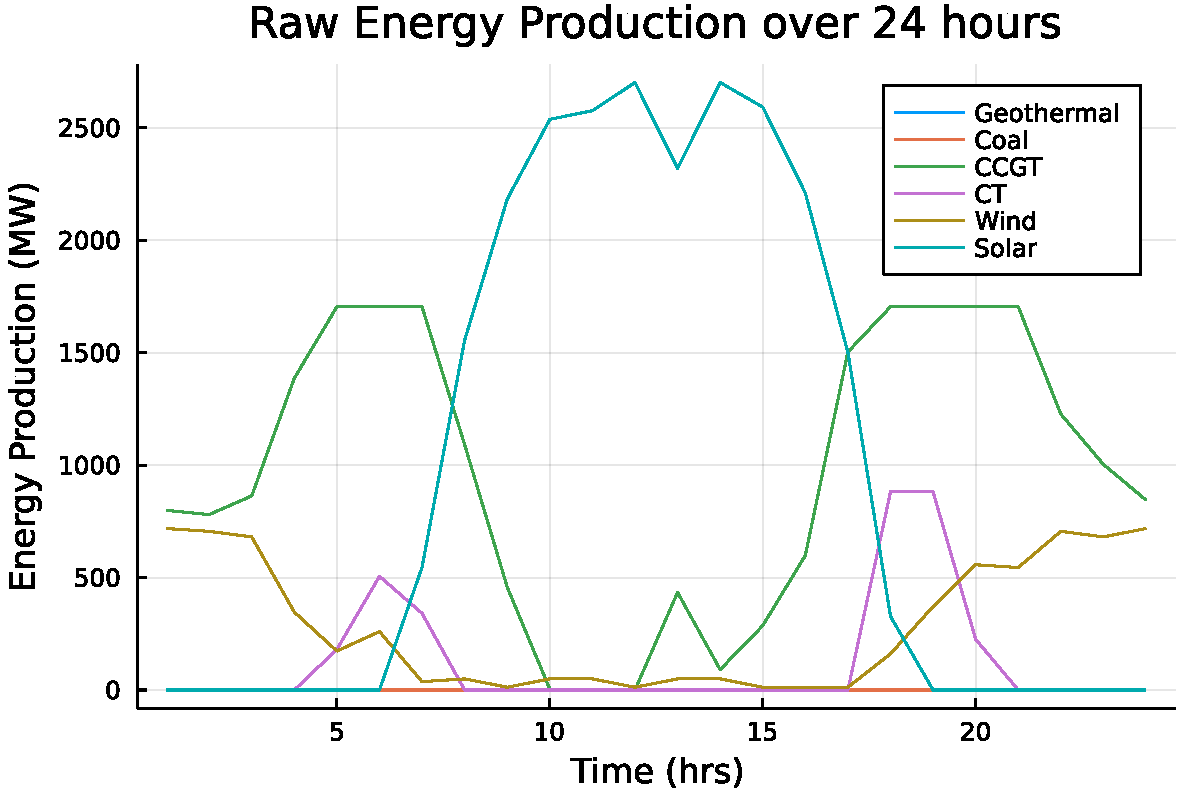
\includegraphics[width=\linewidth]{figures/solution-template_5_1.pdf}

\begin{lstlisting}
(*@\HLJLnB{julia>}@*) (*@\HLJLnf{areaplot}@*)(*@\HLJLp{(}@*)(*@\HLJLn{h}@*)(*@\HLJLoB{{\textquotesingle}}@*)(*@\HLJLp{,}@*)(*@\HLJLn{title}@*) (*@\HLJLoB{=}@*) (*@\HLJLs{"{}Raw}@*) (*@\HLJLs{Energy}@*) (*@\HLJLs{Production}@*) (*@\HLJLs{over}@*) (*@\HLJLs{24}@*) (*@\HLJLs{hours"{}}@*)(*@\HLJLp{,}@*) (*@\HLJLn{xlabel}@*) (*@\HLJLoB{=}@*) (*@\HLJLs{"{}Time}@*) (*@\HLJLs{(hrs)"{}}@*)(*@\HLJLp{,}@*) (*@\HLJLn{ylabel}@*) (*@\HLJLoB{=}@*) (*@\HLJLs{"{}Energy}@*) (*@\HLJLs{Production}@*) (*@\HLJLs{(MW)"{}}@*)(*@\HLJLp{,}@*) (*@\HLJLn{label}@*)(*@\HLJLoB{=}@*) (*@\HLJLp{[}@*)(*@\HLJLs{"{}Geothermal"{}}@*) (*@\HLJLs{"{}Coal"{}}@*) (*@\HLJLs{"{}CCGT"{}}@*) (*@\HLJLs{"{}CT"{}}@*) (*@\HLJLs{"{}Wind"{}}@*) (*@\HLJLs{"{}Solar"{}}@*)(*@\HLJLp{]}@*))
\end{lstlisting}
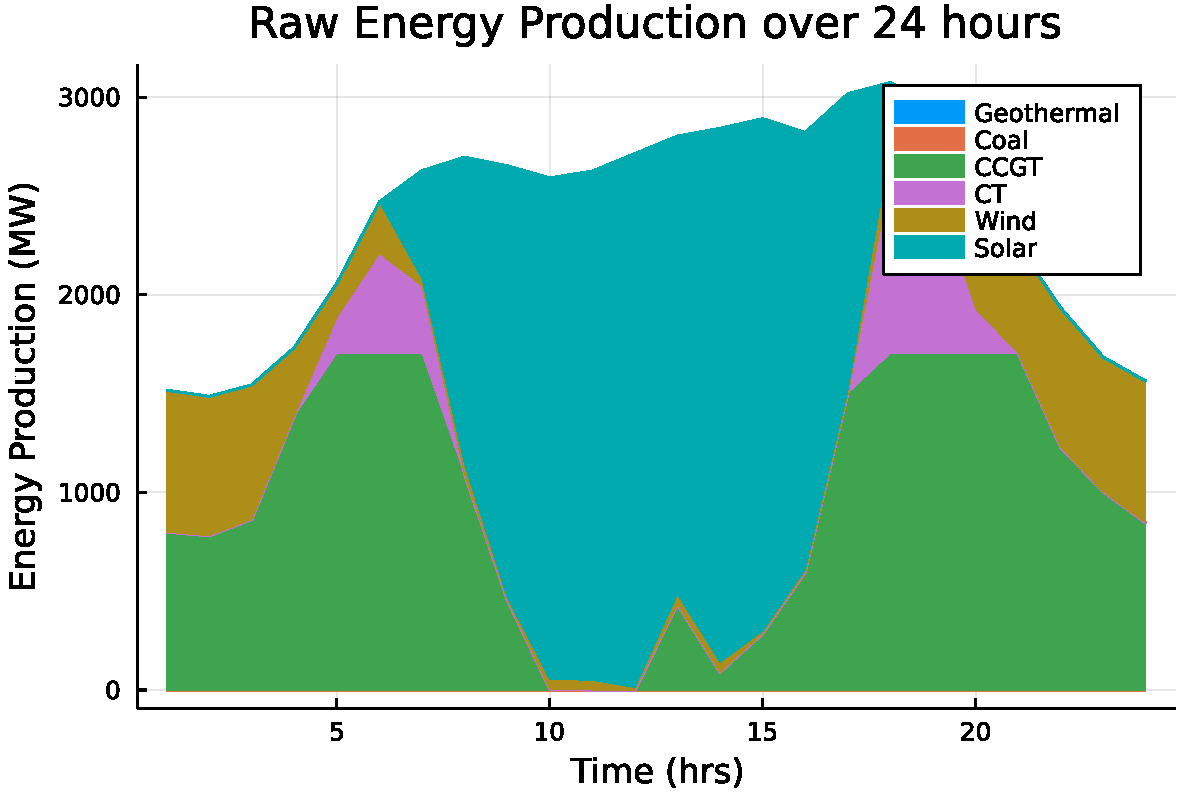
\includegraphics[width=\linewidth]{figures/solution-template_5_2.pdf}

The main takeaways are that solar production dominates during the day while the other 3 forms (CCGT, CT, and Wind) can meet demand when there is less sunlight.

\section{Problem 2}
\subsection{Problem 2.1}
The objective and decision variables would remain the same.

A new constraint would need to be added:

\[
365 \sum_{G}^6 \sum_{t}^{24} CO2_{G} \le 1.5 \text{Mt $CO_2$/yr}
\]
\subsection{Problem 2.2}

\begin{lstlisting}
(*@\HLJLn{L}@*) (*@\HLJLoB{=}@*) (*@\HLJLnf{Model}@*)(*@\HLJLp{(}@*)(*@\HLJLn{HiGHS}@*)(*@\HLJLoB{.}@*)(*@\HLJLn{Optimizer}@*)(*@\HLJLp{)}@*)
(*@\HLJLn{G}@*) (*@\HLJLoB{=}@*) (*@\HLJLni{1}@*)(*@\HLJLoB{:}@*)(*@\HLJLnf{length}@*)(*@\HLJLp{(}@*)(*@\HLJLn{generators}@*)(*@\HLJLp{)}@*)
(*@\HLJLn{T}@*) (*@\HLJLoB{=}@*) (*@\HLJLn{hours}@*)

(*@\HLJLnd{@variable}@*)(*@\HLJLp{(}@*)(*@\HLJLn{L}@*)(*@\HLJLp{,}@*) (*@\HLJLn{x}@*)(*@\HLJLp{[}@*)(*@\HLJLn{G}@*)(*@\HLJLp{]}@*) (*@\HLJLoB{>=}@*) (*@\HLJLni{0}@*)(*@\HLJLp{)}@*)
(*@\HLJLnd{@variable}@*)(*@\HLJLp{(}@*)(*@\HLJLn{L}@*)(*@\HLJLp{,}@*) (*@\HLJLn{y}@*)(*@\HLJLp{[}@*)(*@\HLJLn{G}@*)(*@\HLJLp{,}@*) (*@\HLJLn{T}@*)(*@\HLJLp{]}@*) (*@\HLJLoB{>=}@*) (*@\HLJLni{0}@*)(*@\HLJLp{)}@*)

(*@\HLJLnd{@objective}@*)(*@\HLJLp{(}@*)(*@\HLJLn{L}@*)(*@\HLJLp{,}@*) (*@\HLJLn{Min}@*)(*@\HLJLp{,}@*) (*@\HLJLn{investment{\_}cost}@*)(*@\HLJLoB{{\textquotesingle}*}@*)(*@\HLJLn{x}@*) (*@\HLJLoB{+}@*) (*@\HLJLni{365}@*)(*@\HLJLoB{*}@*)(*@\HLJLp{(}@*)(*@\HLJLnf{sum}@*)(*@\HLJLp{(}@*)(*@\HLJLn{op{\_}cost}@*)(*@\HLJLoB{.*}@*)(*@\HLJLn{y}@*)(*@\HLJLp{))}@*) (*@\HLJLoB{+}@*) (*@\HLJLni{1000}@*)(*@\HLJLoB{*}@*)(*@\HLJLni{365}@*)(*@\HLJLoB{*}@*)(*@\HLJLp{(}@*)(*@\HLJLnf{sum}@*)(*@\HLJLp{(}@*)(*@\HLJLn{y}@*)(*@\HLJLp{)}@*) (*@\HLJLoB{-}@*) (*@\HLJLnf{sum}@*)(*@\HLJLp{(}@*)(*@\HLJLn{demand}@*)(*@\HLJLp{)))}@*)

(*@\HLJLnd{@constraint}@*)(*@\HLJLp{(}@*)(*@\HLJLn{L}@*)(*@\HLJLp{,}@*) (*@\HLJLn{availablility}@*)(*@\HLJLp{[}@*)(*@\HLJLn{g}@*) (*@\HLJLkp{in}@*) (*@\HLJLn{G}@*)(*@\HLJLp{,}@*) (*@\HLJLn{t}@*) (*@\HLJLkp{in}@*) (*@\HLJLn{T}@*)(*@\HLJLp{],}@*) (*@\HLJLn{y}@*)(*@\HLJLp{[}@*)(*@\HLJLn{g}@*)(*@\HLJLp{,}@*)(*@\HLJLn{t}@*)(*@\HLJLp{]}@*) (*@\HLJLoB{<=}@*) (*@\HLJLn{cf}@*)(*@\HLJLp{[}@*)(*@\HLJLn{g}@*)(*@\HLJLp{,}@*)(*@\HLJLn{t}@*)(*@\HLJLp{]}@*)(*@\HLJLoB{*}@*)(*@\HLJLn{x}@*)(*@\HLJLp{[}@*)(*@\HLJLn{g}@*)(*@\HLJLp{])}@*)

(*@\HLJLnd{@constraint}@*)(*@\HLJLp{(}@*)(*@\HLJLn{L}@*)(*@\HLJLp{,}@*) (*@\HLJLn{load}@*)(*@\HLJLp{[}@*)(*@\HLJLn{t}@*) (*@\HLJLkp{in}@*) (*@\HLJLn{T}@*)(*@\HLJLp{],}@*) (*@\HLJLnf{sum}@*)(*@\HLJLp{(}@*)(*@\HLJLn{y}@*)(*@\HLJLp{[}@*)(*@\HLJLoB{:}@*)(*@\HLJLp{,}@*) (*@\HLJLn{t}@*)(*@\HLJLp{])}@*) (*@\HLJLoB{==}@*) (*@\HLJLn{demand}@*)(*@\HLJLp{[}@*)(*@\HLJLn{t}@*)(*@\HLJLp{])}@*)

(*@\HLJLnd{@constraint}@*)(*@\HLJLp{(}@*)(*@\HLJLn{L}@*)(*@\HLJLp{,}@*) (*@\HLJLn{co2}@*)(*@\HLJLp{[}@*)(*@\HLJLn{g}@*) (*@\HLJLkp{in}@*) (*@\HLJLn{G}@*)(*@\HLJLp{],}@*) (*@\HLJLni{365}@*)(*@\HLJLoB{*}@*)(*@\HLJLnf{sum}@*)(*@\HLJLp{((}@*)(*@\HLJLn{co2{\_}emissions}@*)(*@\HLJLp{[}@*)(*@\HLJLn{g}@*)(*@\HLJLp{]}@*)(*@\HLJLoB{*}@*)(*@\HLJLnf{sum}@*)(*@\HLJLp{(}@*)(*@\HLJLn{y}@*)(*@\HLJLp{[}@*)(*@\HLJLn{g}@*)(*@\HLJLp{,}@*)(*@\HLJLoB{:}@*)(*@\HLJLp{])))}@*) (*@\HLJLoB{<=}@*) (*@\HLJLnfB{1.5}@*)(*@\HLJLoB{*}@*)(*@\HLJLni{10}@*)(*@\HLJLoB{{\textasciicircum}}@*)(*@\HLJLni{6}@*)(*@\HLJLp{)}@*)
\end{lstlisting}

1-dimensional DenseAxisArray{ConstraintRef{Model, MathOptInterface.ConstraintIndex{MathOptInterface.ScalarAffineFunction{Float64}, MathOptInterface.LessThan{Float64}}, ScalarShape},1,...} with index sets:
    Dimension 1, 1:6
And data, a 6-element Vector{ConstraintRef{Model, MathOptInterface.ConstraintIndex{MathOptInterface.ScalarAffineFunction{Float64}, MathOptInterface.LessThan{Float64}}, ScalarShape}}:
 co2[1] : 0 ≤ 1.5e6
 co2[2] : 365 y[2,1] + 365 y[2,2] + 365 y[2,3] + 365 y[2,4] + 365 y[2,5] + 365 y[2,6] + 365 y[2,7] + 365 y[2,8] + 365 y[2,9] + 365 y[2,10] + 365 y[2,11] + 365 y[2,12] + 365 y[2,13] + 365 y[2,14] + 365 y[2,15] + 365 y[2,16] + 365 y[2,17] + 365 y[2,18] + 365 y[2,19] + 365 y[2,20] + 365 y[2,21] + 365 y[2,22] + 365 y[2,23] + 365 y[2,24] ≤ 1.5e6
 co2[3] : 156.95 y[3,1] + 156.95 y[3,2] + 156.95 y[3,3] + 156.95 y[3,4] + 156.95 y[3,5] + 156.95 y[3,6] + 156.95 y[3,7] + 156.95 y[3,8] + 156.95 y[3,9] + 156.95 y[3,10] + 156.95 y[3,11] + 156.95 y[3,12] + 156.95 y[3,13] + 156.95 y[3,14] + 156.95 y[3,15] + 156.95 y[3,16] + 156.95 y[3,17] + 156.95 y[3,18] + 156.95 y[3,19] + 156.95 y[3,20] + 156.95 y[3,21] + 156.95 y[3,22] + 156.95 y[3,23] + 156.95 y[3,24] ≤ 1.5e6
 co2[4] : 200.75000000000003 y[4,1] + 200.75000000000003 y[4,2] + 200.75000000000003 y[4,3] + 200.75000000000003 y[4,4] + 200.75000000000003 y[4,5] + 200.75000000000003 y[4,6] + 200.75000000000003 y[4,7] + 200.75000000000003 y[4,8] + 200.75000000000003 y[4,9] + 200.75000000000003 y[4,10] + 200.75000000000003 y[4,11] + 200.75000000000003 y[4,12] + 200.75000000000003 y[4,13] + 200.75000000000003 y[4,14] + 200.75000000000003 y[4,15] + 200.75000000000003 y[4,16] + 200.75000000000003 y[4,17] + 200.75000000000003 y[4,18] + 200.75000000000003 y[4,19] + 200.75000000000003 y[4,20] + 200.75000000000003 y[4,21] + 200.75000000000003 y[4,22] + 200.75000000000003 y[4,23] + 200.75000000000003 y[4,24] ≤ 1.5e6
 co2[5] : 0 ≤ 1.5e6
 co2[6] : 0 ≤ 1.5e6


\subsection{Problem 2.3}

\begin{lstlisting}
(*@\HLJLnB{julia>}@*) (*@\HLJLnf{optimize!}@*)(*@\HLJLp{(}@*)(*@\HLJLn{L}@*)(*@\HLJLp{)}@*)
Presolving model
159 rows, 138 cols, 468 nonzeros
159 rows, 138 cols, 468 nonzeros
Presolve : Reductions: rows 159(-15); columns 138(-12); elements 468(-24)
Solving the presolved LP
Using EKK dual simplex solver - serial
  Iteration        Objective     Infeasibilities num(sum)
          0    -2.0818505000e+10 Pr: 24(159062) 0s
        120     9.3398845328e+08 Pr: 0(0) 0s
Solving the original LP from the solution after postsolve
Model   status      : Optimal
Simplex   iterations: 120
Objective value     :  9.3398845328e+08
HiGHS run time      :          0.00

(*@\HLJLnB{julia>}@*) (*@\HLJLn{L}@*) (*@\HLJLoB{=}@*) (*@\HLJLnf{objective{\_}value}@*)(*@\HLJLp{(}@*)(*@\HLJLn{L}@*)(*@\HLJLp{)}@*)
9.339884532803383e8

(*@\HLJLnB{julia>}@*) (*@\HLJLnf{print}@*)(*@\HLJLp{(}@*)(*@\HLJLn{value}@*)(*@\HLJLoB{.}@*)(*@\HLJLp{(}@*)(*@\HLJLn{x}@*)(*@\HLJLp{))}@*)
1-dimensional DenseAxisArray(*@{{\{}}@*)Float64,1,...(*@{{\}}}@*) with index sets:
    Dimension 1, 1:6
And data, a 6-element Vector(*@{{\{}}@*)Float64(*@{{\}}}@*):
    0.0
    0.0
  813.7901170184164
 1551.4733364332083
 2668.6812691819837
 3015.0665129559793
(*@\HLJLnB{julia>}@*) (*@\HLJLn{value}@*)(*@\HLJLoB{.}@*)(*@\HLJLp{(}@*)(*@\HLJLn{y}@*)(*@\HLJLp{)}@*)
2-dimensional DenseAxisArray(*@{{\{}}@*)Float64,2,...(*@{{\}}}@*) with index sets:
    Dimension 1, 1:6
    Dimension 2, 1:24
And data, a 6(*@\ensuremath{\times}@*)24 Matrix(*@{{\{}}@*)Float64(*@{{\}}}@*):
    0.0     0.0    -0.0      -0.0    (*@\ensuremath{\ldots}@*)    -0.0      -0.0      -0.0
    0.0     0.0    -0.0      -0.0         -0.0      -0.0      -0.0
    0.0     0.0    76.2253  813.79       411.852   216.225    15.1649
    0.0     0.0     0.0     171.979        0.0       0.0       0.0
 1517.0  1486.0  1467.77    747.231     1521.15   1467.77   1547.84
   -0.0     0.0    -0.0      -0.0    (*@\ensuremath{\ldots}@*)    -0.0      -0.0      -0.0
\end{lstlisting}

The utility build of each type of generating plant would be no purchase of geothermal and coal, 813.79 MW for CCGT, 1551.47 MW for CT, 2668.68 MW for wind, and 3015.07 MW for solar. (This is shown above in value.(x))

The main difference between this and part 1 is less investment in CCGT, as it produces a lot of carbon emissions, and more investment into wind and solar, which produce no carbon emissions. 

The total cost will be \$933,988,453.28. The slight increase in cost makes sense as renewable energy sources, which are more expensive, are being prioritizes with the emissions limit.  (This is shown above in objective value.)

\subsection{Problem 2.4}

\begin{lstlisting}
(*@\HLJLnB{julia>}@*) (*@\HLJLn{h}@*) (*@\HLJLoB{=}@*) (*@\HLJLnf{zeros}@*)(*@\HLJLp{(}@*)(*@\HLJLni{6}@*)(*@\HLJLp{,}@*)(*@\HLJLni{24}@*)(*@\HLJLp{)}@*)
6(*@\ensuremath{\times}@*)24 Matrix(*@{{\{}}@*)Float64(*@{{\}}}@*):
 0.0  0.0  0.0  0.0  0.0  0.0  0.0  0.0  (*@\ensuremath{\ldots}@*)  0.0  0.0  0.0  0.0  0.0  0.0  0.0
 0.0  0.0  0.0  0.0  0.0  0.0  0.0  0.0     0.0  0.0  0.0  0.0  0.0  0.0  0.0
 0.0  0.0  0.0  0.0  0.0  0.0  0.0  0.0     0.0  0.0  0.0  0.0  0.0  0.0  0.0
 0.0  0.0  0.0  0.0  0.0  0.0  0.0  0.0     0.0  0.0  0.0  0.0  0.0  0.0  0.0
 0.0  0.0  0.0  0.0  0.0  0.0  0.0  0.0     0.0  0.0  0.0  0.0  0.0  0.0  0.0
 0.0  0.0  0.0  0.0  0.0  0.0  0.0  0.0  (*@\ensuremath{\ldots}@*)  0.0  0.0  0.0  0.0  0.0  0.0  0.0

(*@\HLJLnB{julia>}@*) (*@\HLJLk{for}@*) (*@\HLJLn{i}@*) (*@\HLJLoB{=}@*)(*@\HLJLni{1}@*)(*@\HLJLoB{:}@*)(*@\HLJLni{6}@*)
           (*@\HLJLk{for}@*) (*@\HLJLn{j}@*) (*@\HLJLoB{=}@*) (*@\HLJLni{1}@*)(*@\HLJLoB{:}@*)(*@\HLJLni{24}@*)
               (*@\HLJLn{h}@*)(*@\HLJLp{[}@*)(*@\HLJLn{i}@*)(*@\HLJLp{,}@*)(*@\HLJLn{j}@*)(*@\HLJLp{]}@*) (*@\HLJLoB{=}@*) (*@\HLJLn{value}@*)(*@\HLJLoB{.}@*)(*@\HLJLp{(}@*)(*@\HLJLn{y}@*)(*@\HLJLp{)[}@*)(*@\HLJLn{i}@*)(*@\HLJLp{,}@*)(*@\HLJLn{j}@*)(*@\HLJLp{]}@*)
           (*@\HLJLk{end}@*)
       (*@\HLJLk{end}@*)

(*@\HLJLnB{julia>}@*) (*@\HLJLnf{plot}@*)(*@\HLJLp{(}@*)(*@\HLJLn{h}@*)(*@\HLJLoB{{\textquotesingle}}@*)(*@\HLJLp{,}@*)(*@\HLJLn{title}@*) (*@\HLJLoB{=}@*) (*@\HLJLs{"{}Raw}@*) (*@\HLJLs{Energy}@*) (*@\HLJLs{Production}@*) (*@\HLJLs{over}@*) (*@\HLJLs{24}@*) (*@\HLJLs{hours"{}}@*)(*@\HLJLp{,}@*) (*@\HLJLn{xlabel}@*) (*@\HLJLoB{=}@*) (*@\HLJLs{"{}Time}@*) (*@\HLJLs{(hrs)"{}}@*)(*@\HLJLp{,}@*) (*@\HLJLn{ylabel}@*) (*@\HLJLoB{=}@*) (*@\HLJLs{"{}Energy}@*) (*@\HLJLs{Production}@*) (*@\HLJLs{(MW)"{}}@*)(*@\HLJLp{,}@*) (*@\HLJLn{label}@*)(*@\HLJLoB{=}@*) (*@\HLJLp{[}@*)(*@\HLJLs{"{}Geothermal"{}}@*) (*@\HLJLs{"{}Coal"{}}@*) (*@\HLJLs{"{}CCGT"{}}@*) (*@\HLJLs{"{}CT"{}}@*) (*@\HLJLs{"{}Wind"{}}@*) (*@\HLJLs{"{}Solar"{}}@*)(*@\HLJLp{]}@*))
\end{lstlisting}
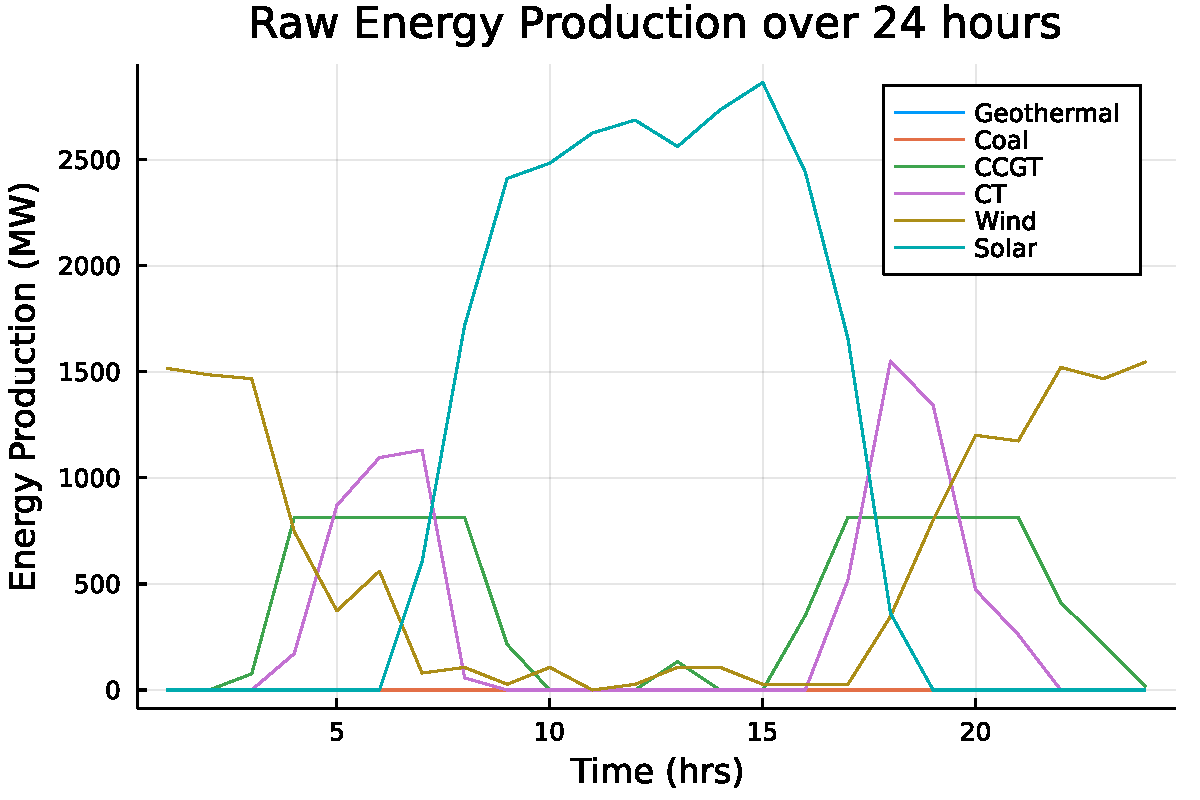
\includegraphics[width=\linewidth]{figures/solution-template_8_1.pdf}

\begin{lstlisting}
(*@\HLJLnB{julia>}@*) (*@\HLJLnf{areaplot}@*)(*@\HLJLp{(}@*)(*@\HLJLn{h}@*)(*@\HLJLoB{{\textquotesingle}}@*)(*@\HLJLp{,}@*)(*@\HLJLn{title}@*) (*@\HLJLoB{=}@*) (*@\HLJLs{"{}Raw}@*) (*@\HLJLs{Energy}@*) (*@\HLJLs{Production}@*) (*@\HLJLs{over}@*) (*@\HLJLs{24}@*) (*@\HLJLs{hours"{}}@*)(*@\HLJLp{,}@*) (*@\HLJLn{xlabel}@*) (*@\HLJLoB{=}@*) (*@\HLJLs{"{}Time}@*) (*@\HLJLs{(hrs)"{}}@*)(*@\HLJLp{,}@*) (*@\HLJLn{ylabel}@*) (*@\HLJLoB{=}@*) (*@\HLJLs{"{}Energy}@*) (*@\HLJLs{Production}@*) (*@\HLJLs{(MW)"{}}@*)(*@\HLJLp{,}@*) (*@\HLJLn{label}@*)(*@\HLJLoB{=}@*) (*@\HLJLp{[}@*)(*@\HLJLs{"{}Geothermal"{}}@*) (*@\HLJLs{"{}Coal"{}}@*) (*@\HLJLs{"{}CCGT"{}}@*) (*@\HLJLs{"{}CT"{}}@*) (*@\HLJLs{"{}Wind"{}}@*) (*@\HLJLs{"{}Solar"{}}@*)(*@\HLJLp{]}@*))
\end{lstlisting}
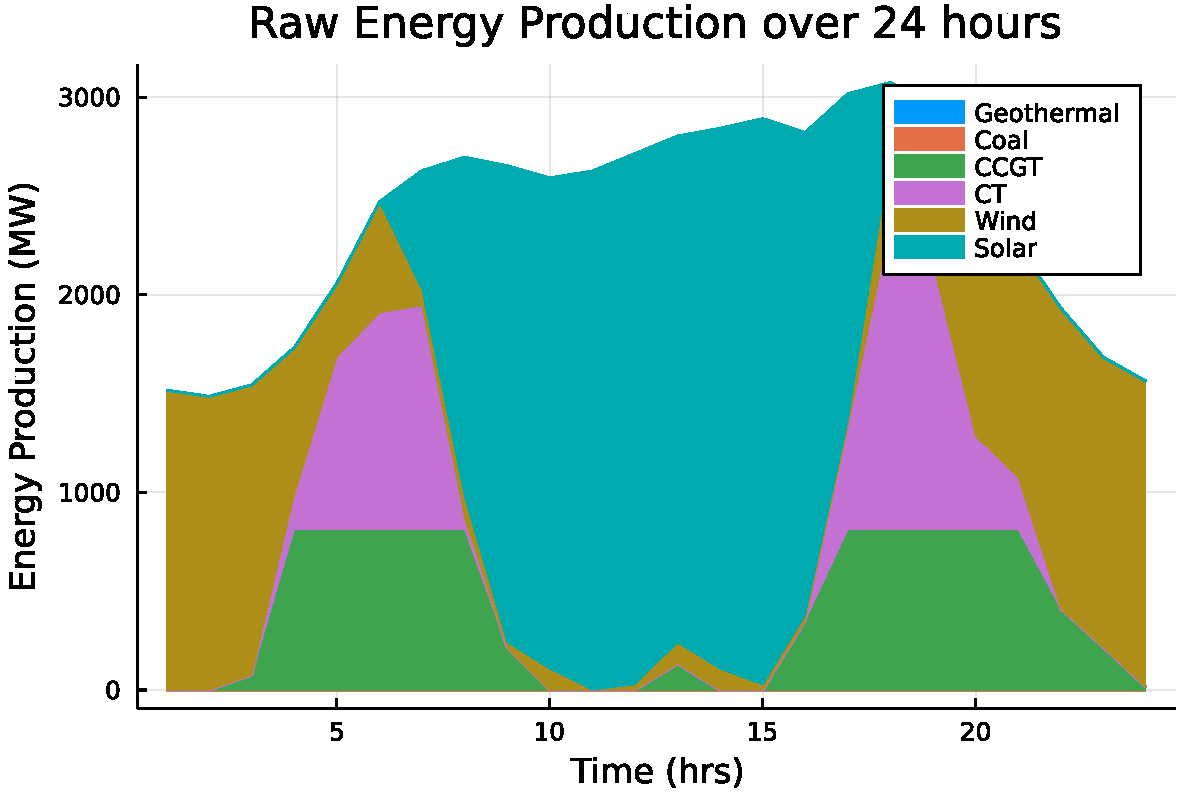
\includegraphics[width=\linewidth]{figures/solution-template_8_2.pdf}

The difference is a major cap or plateau in CCGT production, during peak hours. Renewables also make up a larger proportion of production overall in order to meet the carbon emissiosn requirement. 

\subsection{Problem 2.5}

\begin{lstlisting}
(*@\HLJLnB{julia>}@*) (*@\HLJLn{M}@*) (*@\HLJLoB{=}@*) (*@\HLJLnf{Model}@*)(*@\HLJLp{(}@*)(*@\HLJLn{HiGHS}@*)(*@\HLJLoB{.}@*)(*@\HLJLn{Optimizer}@*)(*@\HLJLp{)}@*)
A JuMP Model
Feasibility problem with:
Variables: 0
Model mode: AUTOMATIC
CachingOptimizer state: EMPTY(*@{{\_}}@*)OPTIMIZER
Solver name: HiGHS

(*@\HLJLnB{julia>}@*) (*@\HLJLn{G}@*) (*@\HLJLoB{=}@*) (*@\HLJLni{1}@*)(*@\HLJLoB{:}@*)(*@\HLJLnf{length}@*)(*@\HLJLp{(}@*)(*@\HLJLn{generators}@*)(*@\HLJLp{)}@*)
1:6

(*@\HLJLnB{julia>}@*) (*@\HLJLn{T}@*) (*@\HLJLoB{=}@*) (*@\HLJLn{hours}@*)
1:24

(*@\HLJLnB{julia>}@*) (*@\HLJLnd{@variable}@*)(*@\HLJLp{(}@*)(*@\HLJLn{M}@*)(*@\HLJLp{,}@*) (*@\HLJLn{x}@*)(*@\HLJLp{[}@*)(*@\HLJLn{G}@*)(*@\HLJLp{]}@*) (*@\HLJLoB{>=}@*) (*@\HLJLni{0}@*)(*@\HLJLp{)}@*)
1-dimensional DenseAxisArray(*@{{\{}}@*)VariableRef,1,...(*@{{\}}}@*) with index sets:
    Dimension 1, 1:6
And data, a 6-element Vector(*@{{\{}}@*)VariableRef(*@{{\}}}@*):
 x[1]
 x[2]
 x[3]
 x[4]
 x[5]
 x[6]

(*@\HLJLnB{julia>}@*) (*@\HLJLnd{@variable}@*)(*@\HLJLp{(}@*)(*@\HLJLn{M}@*)(*@\HLJLp{,}@*) (*@\HLJLn{y}@*)(*@\HLJLp{[}@*)(*@\HLJLn{G}@*)(*@\HLJLp{,}@*) (*@\HLJLn{T}@*)(*@\HLJLp{]}@*) (*@\HLJLoB{>=}@*) (*@\HLJLni{0}@*)(*@\HLJLp{)}@*)
2-dimensional DenseAxisArray(*@{{\{}}@*)VariableRef,2,...(*@{{\}}}@*) with index sets:
    Dimension 1, 1:6
    Dimension 2, 1:24
And data, a 6(*@\ensuremath{\times}@*)24 Matrix(*@{{\{}}@*)VariableRef(*@{{\}}}@*):
 y[1,1]  y[1,2]  y[1,3]  y[1,4]  (*@\ensuremath{\ldots}@*)  y[1,21]  y[1,22]  y[1,23]  y[1,24]
 y[2,1]  y[2,2]  y[2,3]  y[2,4]     y[2,21]  y[2,22]  y[2,23]  y[2,24]
 y[3,1]  y[3,2]  y[3,3]  y[3,4]     y[3,21]  y[3,22]  y[3,23]  y[3,24]
 y[4,1]  y[4,2]  y[4,3]  y[4,4]     y[4,21]  y[4,22]  y[4,23]  y[4,24]
 y[5,1]  y[5,2]  y[5,3]  y[5,4]     y[5,21]  y[5,22]  y[5,23]  y[5,24]
 y[6,1]  y[6,2]  y[6,3]  y[6,4]  (*@\ensuremath{\ldots}@*)  y[6,21]  y[6,22]  y[6,23]  y[6,24]

(*@\HLJLnB{julia>}@*) (*@\HLJLnd{@objective}@*)(*@\HLJLp{(}@*)(*@\HLJLn{M}@*)(*@\HLJLp{,}@*) (*@\HLJLn{Min}@*)(*@\HLJLp{,}@*) (*@\HLJLn{investment{\_}cost}@*)(*@\HLJLoB{{\textquotesingle}*}@*)(*@\HLJLn{x}@*) (*@\HLJLoB{+}@*) (*@\HLJLni{365}@*)(*@\HLJLoB{*}@*)(*@\HLJLp{(}@*)(*@\HLJLnf{sum}@*)(*@\HLJLp{(}@*)(*@\HLJLn{op{\_}cost}@*)(*@\HLJLoB{.*}@*)(*@\HLJLn{y}@*)(*@\HLJLp{))}@*) (*@\HLJLoB{+}@*) (*@\HLJLni{1000}@*)(*@\HLJLoB{*}@*)(*@\HLJLni{365}@*)(*@\HLJLoB{*}@*)(*@\HLJLp{(}@*)(*@\HLJLnf{sum}@*)(*@\HLJLp{(}@*)(*@\HLJLn{y}@*)(*@\HLJLp{)}@*) (*@\HLJLoB{-}@*) (*@\HLJLnf{sum}@*)(*@\HLJLp{(}@*)(*@\HLJLn{demand}@*)(*@\HLJLp{)))}@*)
457000 x[1] + 268000 x[2] + 85000 x[3] + 62580 x[4] + 92000 x[5] + 92000 x[6] + 373030 y[2,1] + 377775 y[3,1] + 381425 y[4,1] + 373030 y[2,2] + 377775 y[3,2] + 381425 y[4,2] + 373030 y[2,3] + 377775 y[3,3] + 381425 y[4,3] + 373030 y[2,4] + 377775 y[3,4] + 381425 y[4,4] + 373030 y[2,5] + 377775 y[3,5] + 381425 y[4,5] + 373030 y[2,6] + 377775 y[3,6] + 381425 y[4,6] + 373030 y[2,7] + 377775 y[3,7] + 381425 y[4,7] + 373030 y[2,8] + 377775 y[3,8] + 381425 y[4,8] + 373030 y[2,9] + 377775 y[3,9] + 381425 y[4,9] + 373030 y[2,10] + 377775 y[3,10] + 381425 y[4,10] + 373030 y[2,11] + 377775 y[3,11] + 381425 y[4,11] + 373030 y[2,12] + 377775 y[3,12] + 381425 y[4,12] + 373030 y[2,13] + 377775 y[3,13] + 381425 y[4,13] + 373030 y[2,14] + 377775 y[3,14] + 381425 y[4,14] + 373030 y[2,15] + 377775 y[3,15] + 381425 y[4,15] + 373030 y[2,16] + 377775 y[3,16] + 381425 y[4,16] + 373030 y[2,17] + 377775 y[3,17] + 381425 y[4,17] + 373030 y[2,18] + 377775 y[3,18] + 381425 y[4,18] + 373030 y[2,19] + 377775 y[3,19] + 381425 y[4,19] + 373030 y[2,20] + 377775 y[3,20] + 381425 y[4,20] + 373030 y[2,21] + 377775 y[3,21] + 381425 y[4,21] + 373030 y[2,22] + 377775 y[3,22] + 381425 y[4,22] + 373030 y[2,23] + 377775 y[3,23] + 381425 y[4,23] + 373030 y[2,24] + 377775 y[3,24] + 381425 y[4,24] + 365000 y[1,1] + 365000 y[5,1] + 365000 y[6,1] + 365000 y[1,2] + 365000 y[5,2] + 365000 y[6,2] + 365000 y[1,3] + 365000 y[5,3] + 365000 y[6,3] + 365000 y[1,4] + 365000 y[5,4] + 365000 y[6,4] + 365000 y[1,5] + 365000 y[5,5] + 365000 y[6,5] + 365000 y[1,6] + 365000 y[5,6] + 365000 y[6,6] + 365000 y[1,7] + 365000 y[5,7] + 365000 y[6,7] + 365000 y[1,8] + 365000 y[5,8] + 365000 y[6,8] + 365000 y[1,9] + 365000 y[5,9] + 365000 y[6,9] + 365000 y[1,10] + 365000 y[5,10] + 365000 y[6,10] + 365000 y[1,11] + 365000 y[5,11] + 365000 y[6,11] + 365000 y[1,12] + 365000 y[5,12] + 365000 y[6,12] + 365000 y[1,13] + 365000 y[5,13] + 365000 y[6,13] + 365000 y[1,14] + 365000 y[5,14] + 365000 y[6,14] + 365000 y[1,15] + 365000 y[5,15] + 365000 y[6,15] + 365000 y[1,16] + 365000 y[5,16] + 365000 y[6,16] + 365000 y[1,17] + 365000 y[5,17] + 365000 y[6,17] + 365000 y[1,18] + 365000 y[5,18] + 365000 y[6,18] + 365000 y[1,19] + 365000 y[5,19] + 365000 y[6,19] + 365000 y[1,20] + 365000 y[5,20] + 365000 y[6,20] + 365000 y[1,21] + 365000 y[5,21] + 365000 y[6,21] + 365000 y[1,22] + 365000 y[5,22] + 365000 y[6,22] + 365000 y[1,23] + 365000 y[5,23] + 365000 y[6,23] + 365000 y[1,24] + 365000 y[5,24] + 365000 y[6,24] - 20818505000

(*@\HLJLnB{julia>}@*) (*@\HLJLnd{@constraint}@*)(*@\HLJLp{(}@*)(*@\HLJLn{M}@*)(*@\HLJLp{,}@*) (*@\HLJLn{availablility}@*)(*@\HLJLp{[}@*)(*@\HLJLn{g}@*) (*@\HLJLkp{in}@*) (*@\HLJLn{G}@*)(*@\HLJLp{,}@*) (*@\HLJLn{t}@*) (*@\HLJLkp{in}@*) (*@\HLJLn{T}@*)(*@\HLJLp{],}@*) (*@\HLJLn{y}@*)(*@\HLJLp{[}@*)(*@\HLJLn{g}@*)(*@\HLJLp{,}@*)(*@\HLJLn{t}@*)(*@\HLJLp{]}@*) (*@\HLJLoB{<=}@*) (*@\HLJLn{cf}@*)(*@\HLJLp{[}@*)(*@\HLJLn{g}@*)(*@\HLJLp{,}@*)(*@\HLJLn{t}@*)(*@\HLJLp{]}@*)(*@\HLJLoB{*}@*)(*@\HLJLn{x}@*)(*@\HLJLp{[}@*)(*@\HLJLn{g}@*)(*@\HLJLp{])}@*)
2-dimensional DenseAxisArray(*@{{\{}}@*)ConstraintRef(*@{{\{}}@*)Model, MathOptInterface.ConstraintIndex(*@{{\{}}@*)MathOptInterface.ScalarAffineFunction(*@{{\{}}@*)Float64(*@{{\}}}@*), MathOptInterface.LessThan(*@{{\{}}@*)Float64(*@{{\}}}@*)(*@{{\}}}@*), ScalarShape(*@{{\}}}@*),2,...(*@{{\}}}@*) with index sets:
    Dimension 1, 1:6
    Dimension 2, 1:24
And data, a 6(*@\ensuremath{\times}@*)24 Matrix(*@{{\{}}@*)ConstraintRef(*@{{\{}}@*)Model, MathOptInterface.ConstraintIndex(*@{{\{}}@*)MathOptInterface.ScalarAffineFunction(*@{{\{}}@*)Float64(*@{{\}}}@*), MathOptInterface.LessThan(*@{{\{}}@*)Float64(*@{{\}}}@*)(*@{{\}}}@*), ScalarShape(*@{{\}}}@*)(*@{{\}}}@*):
 availablility[1,1] : -0.95 x[1] + y[1,1] (*@\ensuremath{\leq}@*) 0.0  (*@\ensuremath{\ldots}@*)  availablility[1,24] : -0.95 x[1] + y[1,24] (*@\ensuremath{\leq}@*) 0.0
 availablility[2,1] : -x[2] + y[2,1] (*@\ensuremath{\leq}@*) 0.0          availablility[2,24] : -x[2] + y[2,24] (*@\ensuremath{\leq}@*) 0.0
 availablility[3,1] : -x[3] + y[3,1] (*@\ensuremath{\leq}@*) 0.0          availablility[3,24] : -x[3] + y[3,24] (*@\ensuremath{\leq}@*) 0.0
 availablility[4,1] : -x[4] + y[4,1] (*@\ensuremath{\leq}@*) 0.0          availablility[4,24] : -x[4] + y[4,24] (*@\ensuremath{\leq}@*) 0.0
 availablility[5,1] : -0.58 x[5] + y[5,1] (*@\ensuremath{\leq}@*) 0.0     availablility[5,24] : -0.58 x[5] + y[5,24] (*@\ensuremath{\leq}@*) 0.0
 availablility[6,1] : y[6,1] (*@\ensuremath{\leq}@*) 0.0               (*@\ensuremath{\ldots}@*)  availablility[6,24] : y[6,24] (*@\ensuremath{\leq}@*) 0.0

(*@\HLJLnB{julia>}@*) (*@\HLJLnd{@constraint}@*)(*@\HLJLp{(}@*)(*@\HLJLn{M}@*)(*@\HLJLp{,}@*) (*@\HLJLn{load}@*)(*@\HLJLp{[}@*)(*@\HLJLn{t}@*) (*@\HLJLkp{in}@*) (*@\HLJLn{T}@*)(*@\HLJLp{],}@*) (*@\HLJLnf{sum}@*)(*@\HLJLp{(}@*)(*@\HLJLn{y}@*)(*@\HLJLp{[}@*)(*@\HLJLoB{:}@*)(*@\HLJLp{,}@*) (*@\HLJLn{t}@*)(*@\HLJLp{])}@*) (*@\HLJLoB{==}@*) (*@\HLJLn{demand}@*)(*@\HLJLp{[}@*)(*@\HLJLn{t}@*)(*@\HLJLp{])}@*)
1-dimensional DenseAxisArray(*@{{\{}}@*)ConstraintRef(*@{{\{}}@*)Model, MathOptInterface.ConstraintIndex(*@{{\{}}@*)MathOptInterface.ScalarAffineFunction(*@{{\{}}@*)Float64(*@{{\}}}@*), MathOptInterface.EqualTo(*@{{\{}}@*)Float64(*@{{\}}}@*)(*@{{\}}}@*), ScalarShape(*@{{\}}}@*),1,...(*@{{\}}}@*) with index sets:
    Dimension 1, 1:24
And data, a 24-element Vector(*@{{\{}}@*)ConstraintRef(*@{{\{}}@*)Model, MathOptInterface.ConstraintIndex(*@{{\{}}@*)MathOptInterface.ScalarAffineFunction(*@{{\{}}@*)Float64(*@{{\}}}@*), MathOptInterface.EqualTo(*@{{\{}}@*)Float64(*@{{\}}}@*)(*@{{\}}}@*), ScalarShape(*@{{\}}}@*)(*@{{\}}}@*):
 load[1] : y[1,1] + y[2,1] + y[3,1] + y[4,1] + y[5,1] + y[6,1] = 1517.0
 load[2] : y[1,2] + y[2,2] + y[3,2] + y[4,2] + y[5,2] + y[6,2] = 1486.0
 load[3] : y[1,3] + y[2,3] + y[3,3] + y[4,3] + y[5,3] + y[6,3] = 1544.0
 load[4] : y[1,4] + y[2,4] + y[3,4] + y[4,4] + y[5,4] + y[6,4] = 1733.0
 load[5] : y[1,5] + y[2,5] + y[3,5] + y[4,5] + y[5,5] + y[6,5] = 2058.0
 load[6] : y[1,6] + y[2,6] + y[3,6] + y[4,6] + y[5,6] + y[6,6] = 2470.0
 load[7] : y[1,7] + y[2,7] + y[3,7] + y[4,7] + y[5,7] + y[6,7] = 2628.0
 load[8] : y[1,8] + y[2,8] + y[3,8] + y[4,8] + y[5,8] + y[6,8] = 2696.0
 load[9] : y[1,9] + y[2,9] + y[3,9] + y[4,9] + y[5,9] + y[6,9] = 2653.0
 load[10] : y[1,10] + y[2,10] + y[3,10] + y[4,10] + y[5,10] + y[6,10] = 2591.0
 (*@\ensuremath{\vdots}@*)
 load[16] : y[1,16] + y[2,16] + y[3,16] + y[4,16] + y[5,16] + y[6,16] = 2821.0
 load[17] : y[1,17] + y[2,17] + y[3,17] + y[4,17] + y[5,17] + y[6,17] = 3017.0
 load[18] : y[1,18] + y[2,18] + y[3,18] + y[4,18] + y[5,18] + y[6,18] = 3074.0
 load[19] : y[1,19] + y[2,19] + y[3,19] + y[4,19] + y[5,19] + y[6,19] = 2957.0
 load[20] : y[1,20] + y[2,20] + y[3,20] + y[4,20] + y[5,20] + y[6,20] = 2487.0
 load[21] : y[1,21] + y[2,21] + y[3,21] + y[4,21] + y[5,21] + y[6,21] = 2249.0
 load[22] : y[1,22] + y[2,22] + y[3,22] + y[4,22] + y[5,22] + y[6,22] = 1933.0
 load[23] : y[1,23] + y[2,23] + y[3,23] + y[4,23] + y[5,23] + y[6,23] = 1684.0
 load[24] : y[1,24] + y[2,24] + y[3,24] + y[4,24] + y[5,24] + y[6,24] = 1563.0

(*@\HLJLnB{julia>}@*) (*@\HLJLnd{@constraint}@*)(*@\HLJLp{(}@*)(*@\HLJLn{M}@*)(*@\HLJLp{,}@*) (*@\HLJLn{co2}@*)(*@\HLJLp{[}@*)(*@\HLJLn{g}@*) (*@\HLJLkp{in}@*) (*@\HLJLn{G}@*)(*@\HLJLp{],}@*) (*@\HLJLni{365}@*)(*@\HLJLoB{*}@*)(*@\HLJLnf{sum}@*)(*@\HLJLp{((}@*)(*@\HLJLn{co2{\_}emissions}@*)(*@\HLJLp{[}@*)(*@\HLJLn{g}@*)(*@\HLJLp{]}@*)(*@\HLJLoB{*}@*)(*@\HLJLnf{sum}@*)(*@\HLJLp{(}@*)(*@\HLJLn{y}@*)(*@\HLJLp{[}@*)(*@\HLJLn{g}@*)(*@\HLJLp{,}@*)(*@\HLJLoB{:}@*)(*@\HLJLp{])))}@*) (*@\HLJLoB{<=}@*) (*@\HLJLnfB{1.501}@*)(*@\HLJLoB{*}@*)(*@\HLJLni{10}@*)(*@\HLJLoB{{\textasciicircum}}@*)(*@\HLJLni{6}@*)(*@\HLJLp{)}@*)
1-dimensional DenseAxisArray(*@{{\{}}@*)ConstraintRef(*@{{\{}}@*)Model, MathOptInterface.ConstraintIndex(*@{{\{}}@*)MathOptInterface.ScalarAffineFunction(*@{{\{}}@*)Float64(*@{{\}}}@*), MathOptInterface.LessThan(*@{{\{}}@*)Float64(*@{{\}}}@*)(*@{{\}}}@*), ScalarShape(*@{{\}}}@*),1,...(*@{{\}}}@*) with index sets:
    Dimension 1, 1:6
And data, a 6-element Vector(*@{{\{}}@*)ConstraintRef(*@{{\{}}@*)Model, MathOptInterface.ConstraintIndex(*@{{\{}}@*)MathOptInterface.ScalarAffineFunction(*@{{\{}}@*)Float64(*@{{\}}}@*), MathOptInterface.LessThan(*@{{\{}}@*)Float64(*@{{\}}}@*)(*@{{\}}}@*), ScalarShape(*@{{\}}}@*)(*@{{\}}}@*):
 co2[1] : 0 (*@\ensuremath{\leq}@*) 1.501e6
 co2[2] : 365 y[2,1] + 365 y[2,2] + 365 y[2,3] + 365 y[2,4] + 365 y[2,5] + 365 y[2,6] + 365 y[2,7] + 365 y[2,8] + 365 y[2,9] + 365 y[2,10] + 365 y[2,11] + 365 y[2,12] + 365 y[2,13] + 365 y[2,14] + 365 y[2,15] + 365 y[2,16] + 365 y[2,17] + 365 y[2,18] + 365 y[2,19] + 365 y[2,20] + 365 y[2,21] + 365 y[2,22] + 365 y[2,23] + 365 y[2,24] (*@\ensuremath{\leq}@*) 1.501e6
 co2[3] : 156.95 y[3,1] + 156.95 y[3,2] + 156.95 y[3,3] + 156.95 y[3,4] + 156.95 y[3,5] + 156.95 y[3,6] + 156.95 y[3,7] + 156.95 y[3,8] + 156.95 y[3,9] + 156.95 y[3,10] + 156.95 y[3,11] + 156.95 y[3,12] + 156.95 y[3,13] + 156.95 y[3,14] + 156.95 y[3,15] + 156.95 y[3,16] + 156.95 y[3,17] + 156.95 y[3,18] + 156.95 y[3,19] + 156.95 y[3,20] + 156.95 y[3,21] + 156.95 y[3,22] + 156.95 y[3,23] + 156.95 y[3,24] (*@\ensuremath{\leq}@*) 1.501e6
 co2[4] : 200.75000000000003 y[4,1] + 200.75000000000003 y[4,2] + 200.75000000000003 y[4,3] + 200.75000000000003 y[4,4] + 200.75000000000003 y[4,5] + 200.75000000000003 y[4,6] + 200.75000000000003 y[4,7] + 200.75000000000003 y[4,8] + 200.75000000000003 y[4,9] + 200.75000000000003 y[4,10] + 200.75000000000003 y[4,11] + 200.75000000000003 y[4,12] + 200.75000000000003 y[4,13] + 200.75000000000003 y[4,14] + 200.75000000000003 y[4,15] + 200.75000000000003 y[4,16] + 200.75000000000003 y[4,17] + 200.75000000000003 y[4,18] + 200.75000000000003 y[4,19] + 200.75000000000003 y[4,20] + 200.75000000000003 y[4,21] + 200.75000000000003 y[4,22] + 200.75000000000003 y[4,23] + 200.75000000000003 y[4,24] (*@\ensuremath{\leq}@*) 1.501e6
 co2[5] : 0 (*@\ensuremath{\leq}@*) 1.501e6
 co2[6] : 0 (*@\ensuremath{\leq}@*) 1.501e6

(*@\HLJLnB{julia>}@*) (*@\HLJLnf{optimize!}@*)(*@\HLJLp{(}@*)(*@\HLJLn{M}@*)(*@\HLJLp{)}@*)
Presolving model
159 rows, 138 cols, 468 nonzeros
159 rows, 138 cols, 468 nonzeros
Presolve : Reductions: rows 159(-15); columns 138(-12); elements 468(-24)
Solving the presolved LP
Using EKK dual simplex solver - serial
  Iteration        Objective     Infeasibilities num(sum)
          0    -2.0818505000e+10 Pr: 24(159062) 0s
        120     9.3393330482e+08 Pr: 0(0) 0s
Solving the original LP from the solution after postsolve
Model   status      : Optimal
Simplex   iterations: 120
Objective value     :  9.3393330482e+08
HiGHS run time      :          0.00

(*@\HLJLnB{julia>}@*) (*@\HLJLn{M}@*) (*@\HLJLoB{=}@*) (*@\HLJLnf{objective{\_}value}@*)(*@\HLJLp{(}@*)(*@\HLJLn{M}@*)(*@\HLJLp{)}@*)
9.339333048215866e8

(*@\HLJLnB{julia>}@*) (*@\HLJLnf{print}@*)(*@\HLJLp{(}@*)(*@\HLJLn{value}@*)(*@\HLJLoB{.}@*)(*@\HLJLp{(}@*)(*@\HLJLn{x}@*)(*@\HLJLp{))}@*)
1-dimensional DenseAxisArray(*@{{\{}}@*)Float64,1,...(*@{{\}}}@*) with index sets:
    Dimension 1, 1:6
And data, a 6-element Vector(*@{{\{}}@*)Float64(*@{{\}}}@*):
    0.0
    0.0
  813.824069940046
 1551.7793552294854
 2666.040442264474
 3015.0943111340584
(*@\HLJLnB{julia>}@*) (*@\HLJLn{value}@*)(*@\HLJLoB{.}@*)(*@\HLJLp{(}@*)(*@\HLJLn{y}@*)(*@\HLJLp{)}@*)
2-dimensional DenseAxisArray(*@{{\{}}@*)Float64,2,...(*@{{\}}}@*) with index sets:
    Dimension 1, 1:6
    Dimension 2, 1:24
And data, a 6(*@\ensuremath{\times}@*)24 Matrix(*@{{\{}}@*)Float64(*@{{\}}}@*):
    0.0     0.0    -0.0      -0.0    (*@\ensuremath{\ldots}@*)    -0.0      -0.0      -0.0
    0.0     0.0    -0.0      -0.0         -0.0      -0.0      -0.0
    0.0     0.0    77.6778  813.824      413.357   217.678    16.6965
    0.0     0.0     0.0     172.685        0.0       0.0       0.0
 1517.0  1486.0  1466.32    746.491     1519.64   1466.32   1546.3
   -0.0     0.0    -0.0      -0.0    (*@\ensuremath{\ldots}@*)    -0.0      -0.0      -0.0

(*@\HLJLnB{julia>}@*) (*@\HLJLnf{print}@*)(*@\HLJLp{(}@*)(*@\HLJLn{M}@*)(*@\HLJLoB{-}@*)(*@\HLJLn{L}@*)(*@\HLJLp{)}@*)
-55148.45875167847
\end{lstlisting}

The model was run again this time with the slight increase to the carbon emission constraint.

Allowing an extra 1000tCO2/yr decreases the optimal cost to the utility by \$55,148. 

\section{References}
Alex Wang Grace Lin



\end{document}